% =====================================================================
\section{What was tried and dropped}
\label{sec:dropped}

Most of what was tried did not stay. The searches of Section~\ref{sec:loop} kept
a small share of the changes they ran (Table~\ref{tab:loop}); every change tried
alone in the first round is in Figure~\ref{fig:loopheat}, and the losses tried in
the first revision are in Table~\ref{tab:losses}. Table~\ref{tab:dropped} lists
the larger things the revision tried beyond the searches and did not keep, and
when each becomes worth trying again.

\begin{table*}[t]
\centering
\caption{\textbf{What the revision tried beyond the searches and did not keep.}
Each was written down before it ran.}
\label{tab:dropped}
\footnotesize
\renewcommand{\arraystretch}{1.15}
\begin{tabular}{p{0.25\textwidth}p{0.36\textwidth}p{0.31\textwidth}}
\toprule
\textbf{Tried} & \textbf{What happened} & \textbf{Worth revisiting when} \\
\midrule
Count likelihoods that treat zero weeks on their own (negative binomial, zero-inflated, hurdle), on the world model & Kept on M5 and Favorita (hurdle) and snacks (negative binomial); nothing on the other six data sets & Lines are slower or more often out of stock than here \\
Pretraining the world model's encoder on the latent objective, then fitting the forecast at a lower rate & Kept on snacks only, on the search windows; with nothing kept on eight of nine data sets, Favorita's rerun on its final loss was stopped early & More unlabelled history is available than the forecast needs, as across many categories \\
Training on other retailers' data with each own data set (RQ4) & Helped neither model by more than \rqPoolGainMax{} on any data set, and hurt LightGBM most & The other data come from the same retailer or the same categories \\
The world model alone for series with less than 26 weeks of history & No better than the average on lines with history; worse on snacks & A longer history threshold is set from a retailer's own range data \\
Weights fitted to earlier windows in place of equal weights & Reported in Section~\ref{sec:support} & Many more windows are available to fit them on \\
Timestral in place of TimesFM in the three-model ensemble & Reported in Section~\ref{sec:support} & A retail-trained version is released \\
\bottomrule
\end{tabular}
\end{table*}

The first version of this paper also tried a stock term for the dip after a
promotion, extra loss weight on the periods after a promotion, and a graph model
sharing information between stores; none was kept, and they were not run again on
the tuned models. Their record is in the first version; the loss experiments among them are in
Figure~\ref{fig:sup-devlosses}.

\subsection{Losses and pretraining explored}
\label{sec:sup-explore}

\textbf{Count likelihoods helped on three data sets and JEPA pretraining on one;
the plain loss stayed everywhere else.} After each search, the world model had a
round of count likelihoods and a round of JEPA pretraining
(Section~\ref{sec:loop}). The likelihood round screened \sfLossTried{}
likelihoods on each of \sfLossSets{} data sets with one seed each, \sfLossScreens{}
screens in all, of which \sfLossScreenBetter{} came in below the starting score;
the best went on to three seeds, and a change was kept only where it beat the
start by more than the keep bar (Figure~\ref{fig:sup-explore}a and
Table~\ref{tab:sup-explore}). It was kept on \sfLossKeptSets{}: \sfLossKeptNames{}.
The JEPA round pretrained the encoder on the latent term alone
(Section~\ref{sec:losses}), for a short and a long run, then fitted the forecast
at a lower rate. Of its \sfJepaScreens{}
screens, \sfJepaScreenBetter{} came in below the start, and it was kept on
\sfJepaKeptNames{} only (Figure~\ref{fig:sup-explore}b).

The first version tried \sfDevChanges{} changes to the world model's loss in
\sfDevRuns{} runs on the development windows, \sfDevScored{} of them scored
against the settings they changed (Figure~\ref{fig:sup-devlosses}); the other
\sfDevNotRun{} were not run on the full data. \sfDevBetter{} of the
\sfDevScored{} lowered the error. Latent pretraining and the latent term, in
every form tried, moved the score by at most \sfDevLatentMax{} either way. Extra
weight on the periods after a promotion and the combined peak, dollar and
Tweedie weighting moved it most, in both directions: every form helped cheese
and hurt snacks and analgesics, so none was kept for every category.
The settings searches of Section~\ref{sec:loop} then tried the loss weights again
one at a time on each data set (Figure~\ref{fig:loopheat}).

\begin{table*}[t]
\centering\footnotesize\setlength{\tabcolsep}{4pt}
\caption{Every likelihood and JEPA pretraining recipe tried on the tuned world model, WRMSSE on the search windows.
Start: the settings each round began from.
A number in brackets is a one-seed screen that did not earn a three-seed try; a plain number is the three-seed mean;
bold marks the change kept, which had to beat the start by more than the keep bar on the search windows.}
\label{tab:sup-explore}
\begin{adjustbox}{max width=\textwidth}\begin{tabular}{l ccccc ccc}
\toprule
 & \multicolumn{5}{c}{Likelihood round} & \multicolumn{3}{c}{JEPA pretraining round}\\
\cmidrule(lr){2-6}\cmidrule(lr){7-9}
Data set & Start & NB & NB, spread by item & ZINB, spread by item & Hurdle NB, spread by item & Start & Short & Long\\
\midrule
Analgesics & 0.509 & (0.518) & (0.515) & (0.518) & (0.539) & 0.509 & 0.511 & (0.537) \\
Bottled juice & 0.587 & (0.592) & (0.601) & (0.614) & (0.604) & 0.587 & (0.635) & (0.615) \\
Cheese & 0.392 & (0.450) & 0.403 & 0.396 & 0.382 & 0.392 & (0.401) & (0.406) \\
Frozen entrees & 0.216 & 0.214 & 0.218 & 0.215 & 0.216 & 0.216 & (0.267) & (0.255) \\
Soft drinks & 0.572 & (0.613) & (0.604) & (0.606) & (0.598) & 0.572 & 0.612 & (0.603) \\
Snacks & 0.439 & (0.481) & \textbf{0.420} & 0.427 & 0.429 & 0.420 & (0.428) & \textbf{0.400} \\
Frat & 0.547 & (0.584) & (0.600) & (0.585) & (0.590) & 0.547 & (0.572) & (0.566) \\
M5 & 0.547 & (0.553) & (0.558) & 0.552 & \textbf{0.533} & 0.533 & (0.537) & (0.544) \\
Favorita & 0.483 & 0.488 & (0.476) & 0.469 & \textbf{0.468} & 0.483 & (0.527) & (0.523) \\
\bottomrule
\end{tabular}\end{adjustbox}
\end{table*}


\begin{figure*}[t]
\centering
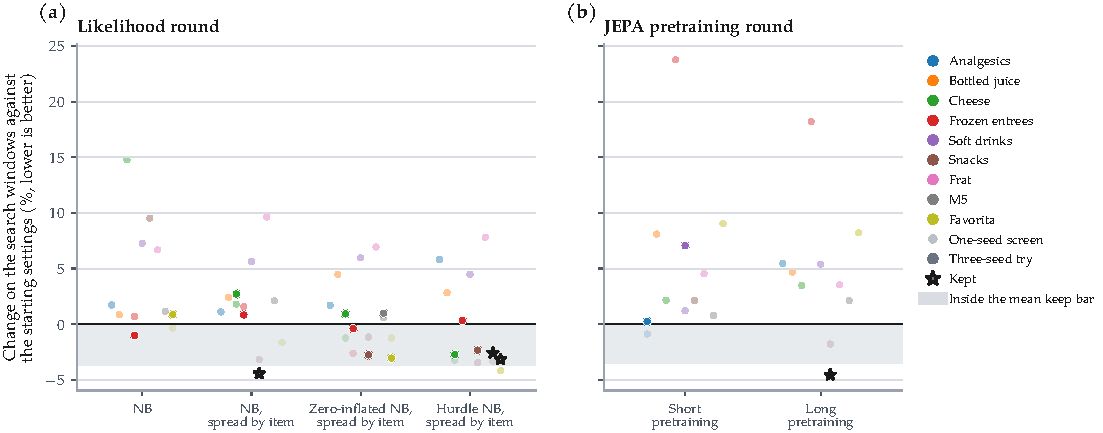
\includegraphics[width=\textwidth]{figs/fig_sup_explore.pdf}
\caption{The likelihood and JEPA pretraining rounds of the tuned world model.
Change in WRMSSE on the search windows against the settings each round started
from, for each one-seed screen (faint) and three-seed try (solid); stars mark the
change kept. A change was kept only where its three-seed mean beat the start by
more than the keep bar; the grey band is the mean keep bar over data sets.}
\label{fig:sup-explore}
\end{figure*}

\begin{figure*}[t]
\centering
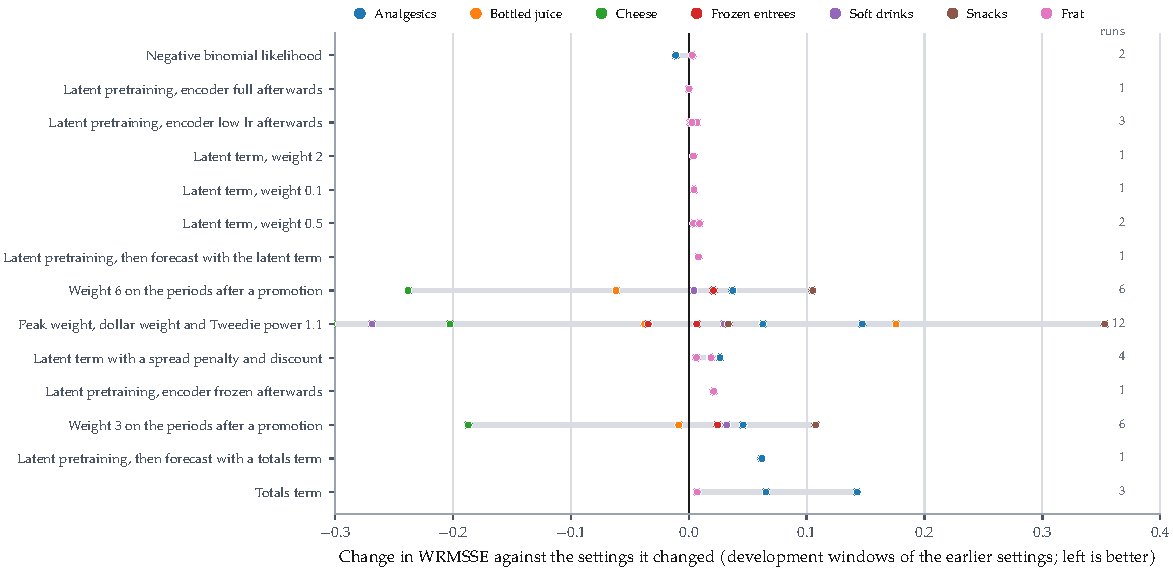
\includegraphics[width=\textwidth]{figs/fig_sup_devlosses.pdf}
\caption{Every loss change of the first version against the settings it changed,
on the development windows. Each dot is one run, coloured by data set; the bar
spans the runs of a change, and the right-hand column counts them. Changes not
run on the full data are not shown.}
\label{fig:sup-devlosses}
\end{figure*}

